\chapter{GIỚI THIỆU}
\label{ch:gioi-thieu}

% --- 1.1 Bối cảnh và lý do chọn đề tài ---
\section{Giới thiệu chung}
\label{sec:boi-canh-ly-do}

Lừa  đảo  trực  tuyến  (phishing)  là  một  loại  hình  lừa  đảo  trực  tuyến  trong  đó  một  trang  web  độc  hại  cố  gắng  lừa  đảo  người  dùng  bằng  cách  giả  mạo  danh  tính.
tự  nhận  mình  là  một  trang  web  hợp  pháp  để  lấy  thông  tin  nhạy  cảm  như  mật  khẩu,  chi  tiết  tài  khoản,
hoặc  thông  tin  ngân  hàng. Theo các báo cáo an ninh mạng gần đây, số lượng các vụ tấn công phishing tăng trưởng nhanh về số lượng theo cấp số nhân với các hình thức ngày càng đa dạng một số hình thức mới đáng chú ý như phishing qua email, CEO Phishing nhắm vào những người có vị trí quan trọng trong tổ chức, doanh nghiệp, QR Phishing, gây thiệt hại hàng tỷ USD mỗi năm  trên toàn cầu nhần mạnh một giải pháp tiến bộ và hiệu quả ~\cite{chargebacks911}.

Một  trong  những  thách  thức  khó  khăn  nhất  trong  an  ninh  mạng  hiện  nay  là  bảo  vệ và chống  lại  các  cuộc  tấn  công  lừa  đảo do kẻ  tấn  công  lừa  đảo  sử  dụng  nhiều  kỹ  thuật  khác  nhau  để
lừa  người  dùng  truy  cập  vào  các  trang  web  giả  mạo, chẳng hạn như đe dọa tạm ngưng tài khoản khách hàng trong trường hợp họ không hoàn tất quy trình nâng cấp tài khoản, yêu cầu người dùng cung cấp một số thông tin bổ sung để xác minh tài khoản của họ, hoặc các mục đích khác. Điều  này  cho  phép  tội  phạm  mạng  lấy được thông  tin  
nhạy  cảm  và  chiếm  đoạt  tiền  mà  không  được  phép. Cùng với sự phát triển của hạ tầng Internet   các  chiến  dịch  lừa  đảo  trực  tuyến  có  thể  được  thực  hiện được  triển  khai  khá  thuận  tiện  từ  bất  cứ  đâu  trên  thế  giới.  Việc  tạo  ra  một liên kết giả mạo dễ  hơn  nhiều  so  với  việc  xâm  nhập  vào  hệ  thống  an  ninh. Tấn  công  lừa  đảo  vẫn  
là  một  cuộc  tấn  công  mạng  nổi  bật  và  hiệu  quả,  cho  thấy  sự  tăng  trưởng  
ổn  định  qua  nhiều  năm.  Theo  dữ  
liệu  được  được VPNRanks quan sát trong năm năm qua. số  lượng  các  cuộc  tấn  công  lừa  đảo  trên  web  
độc  nhất  được  phát  hiện năm  2025  là  1.081.373,  tăng  từ  880.418 
trong  năm 2023,  như  được  minh  họa  trong .  Dữ  liệu  này  cho  
thấy  xu  hướng  gia  tăng  của  các  cuộc  tấn  công  lừa  đảo. 
\begin{figure}[htbp]
    \centering
    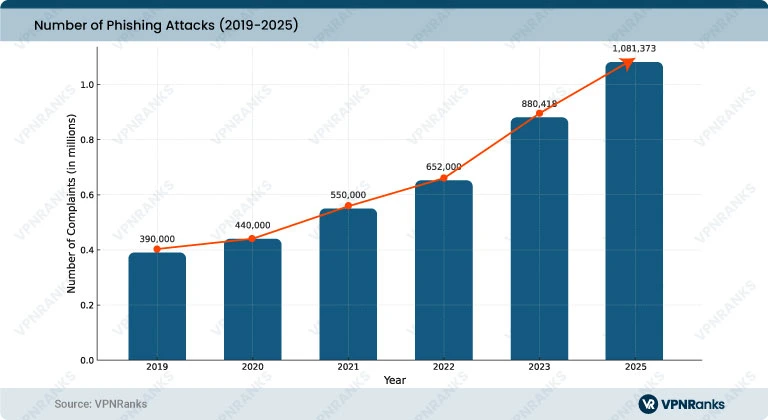
\includegraphics[width=0.9\textwidth]{figures/hinh1.1.png} 
    \caption{Xu hướng tấn công trực tuyến trong năm năm (2019-2025).}
    \label{figures/kien-truc-extension}
\end{figure}


\section{Động lực}
Hiện nay, nhiều phương pháp phòng chống phishing đã được triển khai, trong đó blacklist (danh sách đen) là một trong những kỹ thuật phổ biến nhất. Tuy nhiên, các phương pháp này vẫn tồn tại nhiều hạn chế do phụ thuộc vào cơ sở dữ liệu các trang web độc hại đã được phát hiện trước đó. Trong khi đó, các website phishing mới liên tục xuất hiện với nhiều hình thức ngụy trang ngày càng tinh vi nhằm vượt qua các cơ chế phát hiện truyền thống. Bên cạnh đó, các bộ dữ liệu chuẩn phục vụ huấn luyện mô hình thường không được cập nhật thường xuyên, gây khó khăn trong việc thích ứng với các xu hướng tấn công mới.

Trước thực tế đó cùng sự phát triển của các phương pháp học máy (Machine Learning) và học sâu (Deep Learning) đã mở ra hướng tiếp cận hiệu quả trong việc phát hiện và nhận diện các URL độc hại. Khả năng học đặc trưng từ dữ liệu và phát hiện mẫu bất thường của các mô hình trí tuệ nhân tạo giúp tăng độ chính xác trong nhận diện phishing, đồng thời hỗ trợ cảnh báo sớm cho người dùng trước khi truy cập vào các trang web nguy hiểm.

Xuất phát từ nhu cầu thực tiễn về bảo vệ người dùng trong môi trường trực tuyến, việc phát triển một công cụ hỗ trợ nhận diện liên kết phishing ngay trên trình duyệt web là hết sức cần thiết. Vì vậy, đề tài “Xây dựng hệ thống phát hiện trang web lừa đảo dựa trên mô hình trí tuệ nhân tạo” được lựa chọn nhằm kết hợp khả năng bảo vệ thời gian thực với sức mạnh phân tích của mô hình AI. Giải pháp này hướng tới việc xây dựng một lớp phòng thủ chủ động, giúp người dùng nhận diện sớm các nguy cơ lừa đảo, hạn chế rủi ro mất mát dữ liệu cá nhân và nâng cao mức độ an toàn khi sử dụng Internet.

\section{Mục tiêu và giải pháp}
\label{sec:muc-tieu-pham-vi}
\subsection{Mục tiêu }
   Mục tiêu chính của khóa luận này là nghiên cứu và phát triển một tiện ích mở rộng trên trình duyệt nhằm tự động nhận diện và đưa ra cảnh báo kịp thời về các liên kết lừa đảo xuất hiện trong các tin nhắn và bài đăng trên các nền tảng mạng xã hội. Mục tiêu này được hiện thực hóa trên sản phẩm thông qua hai chức năng chính: chức năng bảo mật chủ động tập trung vào việc tự động rà soát, trích xuất và kiểm định độ tin cậy của toàn bộ liên kết hiện diện trong nội dung trang web ngay tại thời điểm người dùng truy cập  và chức năng hỗ trợ và xác thực tương tác cung cấp cho người dùng công cụ để chủ động kiểm tra tính xác thực của một đường dẫn cụ thể thông qua giao diện tiện ích.

\subsection{Giải pháp}

    Để hiện thực hóa các mục tiêu đề ra, tiện ích CheckPost xây dựng hệ thống phát hiện phishing theo thời gian thực theo mô hình client-sever hỗ trợ các tình năng đã nêu ở trên sử dụng các giải pháp kỹ thuật trọng tâm:giám sát động tự động quét trang đang sử bằng Mutation Observer để theo dõi sự thay đổi của cây cấu trúc DOM giúp phát hiện các liên kết mới khi người dùng cuộn trang trên X hoặc các nền tảng SPA (Single Page Application) gửi về phía máy chủ backend. triển khai thuật toán học máy tại phía sever Sử dụng kỹ thuật UI Injection để chèn trực tiếp các nhãn cảnh báo và lớp phủ cảnh bảo vào giao diện bài đăng, giúp người dùng nhận biết rủi ro mà không cần thao tác
% --- 1.4 Cấu trúc khóa luận ---
\section{Kết quả}
Tiện ích CheckPost là sản phẩm của khóa luận, hỗ trợ đầy đủ các tính năng
 với độ chính xác và độ tin cậy cao, cụ thể bao gồm:
 
• Về hiệu năng: Tuy hỗ trợ nhiều chức năng, CheckPost không gây ảnh
hưởng tiêu cực đến trải nghiệm của người dùng. Tuy thời gian chạy script
tăng do số lượng lớn JavaScript CheckPost sử dụng, thời gian tải trang và
hiển thị trang không bị ảnh hưởng.

• Về các mô hình học máy: Mô hình lõi sử dụng thuật toán học máy kết hợp (Ensemble Learning) với cốt lõi là \textbf{XGBoost} kết hợp cùng \textbf{Heuristic Engine}. Hệ thống cho kết quả phân loại với độ chính xác và tính khái quát hóa cực cao nhờ quá trình làm sạch rò rỉ dữ liệu (Data Leakage) nghiêm ngặt trên tập dữ liệu lớn. Đặc biệt, hệ thống còn cung cấp khả năng giải thích dự đoán (Explainable AI), giúp minh bạch hóa các quyết định ngăn chặn.
\section{Cấu trúc của khóa luận}
\label{sec:cau-truc-kl}

Khóa luận được cấu trúc gồm các chương như sau:

\begin{description}
    \item[Chương 2 - Cơ sở lý thuyết:] Tổng quan về các kiến thức nền tảng được
sử dụng để xây dựng tiện ích, bao gồm kiến trúc của tiện ích, kỹ thuật giám sát và trích xuất dữ liệu Web động tổng quan về các thuật toán học máy và kiến trúc tiện ích trình duyệt.
    \item[Chương 3 - Tiện ích CheckPost:] Phân tích cụ thể tiện íchtừ kiến trúc tổng quát tới cách thức hoạt động,từ kiến trúc tổng quát tới cách thức hoạt động,
    \item[Chương 4 - Đánh giá:] Chi tiết quá trình huấn luyện mô hình, kết quả thực nghiệm trên các tập dữ liệu mẫu.
    \item[Chương 5 - Kết luận và Hướng phát triển:] Tổng kết các kết quả đạt được, chỉ ra các hạn chế và đề xuất hướng cải thiện trong tương lai.
\end{description}